\documentclass[a4paper,12pt]{article}
\usepackage[utf8]{inputenc}
\usepackage[ngerman]{babel}
\usepackage{geometry}
\usepackage{graphicx}
\usepackage{xcolor}
\usepackage{amsmath}
\usepackage{hyperref}
\usepackage{float}
\usepackage{subcaption}
\geometry{a4paper, left=2.5cm, right=2.5cm, top=2.5cm, bottom=2.5cm}


\title{Abgabe 1 Computergestützte Methoden}
\author{Clieven Roham(4356033), Kerim Kartal(4360686), Christian Krifo (4351512)}
\date{24.11.2024}
\begin{document}
\maketitle
\tableofcontents
\section{Der zentrale Grenzwertsatz}

Der zentrale Grenzwertsatz (ZGS) ist ein fundamentales Resultat der Wahrscheinlichkeitstheorie, das
die Verteilung von Summen unabhängiger, identisch verteilter (i.i.d.) Zufallsvariablen (ZV) beschreibt.
Er besagt, dass unter bestimmten Voraussetzungen die Summe einer großen Anzahl solcher ZV
annähernd normalverteilt ist, unabhängig von der Verteilung der einzelnen ZV. Dies ist besonders
nützlich, da die Normalverteilung gut untersucht und mathematisch handhabbar ist.

\subsection{Aussage}
Sei $X_1, X_2, \ldots, X_n$ eine Folge von i.i.d. ZV mit dem Erwartungswert $\mu = E(X_i)$ und der
Varianz $\sigma^2 = \text{Var}(X_i)$, wobei $0 < \sigma^2 < \infty$ gelte. Dann konvergiert die
standardisierte Summe $Z_n$ dieser ZV für $n \to \infty$ in Verteilung gegen eine
Standardnormalverteilung:
\[
Z_n = \frac{\sum_{i=1}^n X_i - n\mu}{\sigma\sqrt{n}} \xrightarrow{d} N(0,1).
\]
Das bedeutet, dass für große $n$ die Summe der ZV näherungsweise normalverteilt ist mit
Erwartungswert $n\mu$ und Varianz $n\sigma^2$:
\[
\sum_{i=1}^n X_i \sim N(n\mu, n\sigma^2).
\]
\subsection{Erklärung der Standardisierung}

Um die Summe der ZV in eine Standardnormalverteilung zu transformieren, subtrahiert man den
Erwartungswert $n\mu$ und teilt durch die Standardabweichung $\sigma\sqrt{n}$. Dies führt zu der
obigen Formel (1). Die Darstellung (2) ist für $n \to \infty$ nicht wohldefiniert.
\subsection{Anwendungen}
Der ZGS wird in vielen Bereichen der Statistik und der Wahrscheinlichkeitstheorie angewendet.
Typische Beispiele sind:

\begin{itemize}
    \item Prognose in der Wirtschaft:\\
     Nehmen wir an, dass ein Einzelhändler die durchschnittliche Ausgabenhöhe pro Kunde an einem Tag prognostizieren möchte, wobei jeder Kunde einen zufälligen Betrag ausgibt. Somit könnte die Verteilung dieser Beiträge stark variieren. Durch den zentralen Grenzwertsatz können die Mittelwerte der Ausgaben über viele Kunden als normalverteilt angenommen werden. Dies erleichtert die Vorhersage des durchschnittlichen Umsatzes und das Modellieren von Risiken.
 \item Qualitätskontrolle in der Produktion:\\
 In einem weiteren Anwendungsbeispiel könnte man annehmen, dass ein Unternehmen in der Produktion von Glühbirnen, sicherstellen möchte, dass die Glühbirnen im Durchschnitt eine bestimmte Lebensdauer haben. Jede einzelne Glühbirne kann eine unterschiedliche Lebensdauer haben, die einer unbekannten Verteilung folgt.
Durch den zentralen Grenzwertsatz kann der Mittelwert der Lebensdauern einer Stichprobe als näherungsweise normalverteilt betrachtet werden. Das Unternehmen kann so Hypothesentests durchführen oder Abweichungen vom Sollwert leichter identifizieren.

\end{itemize}

\section{Bearbeitung Aufgabe 1}

\subsection{Höchste mittlere Temperatur}

Zu Beginn haben wir den gegebenen Datensatz in eine Tabellenkalkulation von Excel importiert. Darauf filterten wir nach unserem gruppenspezifischen Datensatz, die 64. 

\begin{figure}[h]
    \centering
    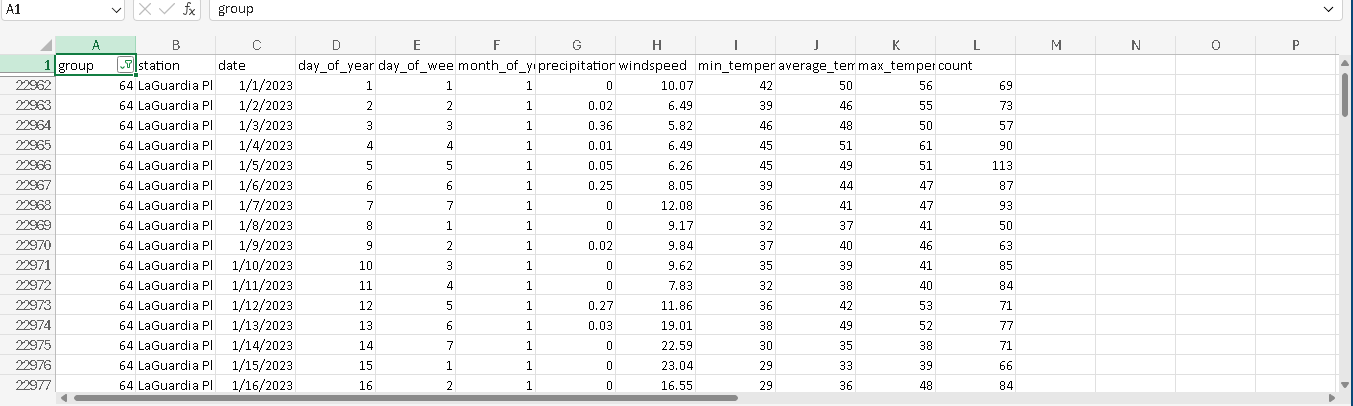
\includegraphics[width=1\linewidth]{Excel1.PNG}
    \caption{Sortierung}
    \label{fig:enter-label}
\end{figure}

\subsection{Tabellenkalkulation}
\textbf{Berechnung der höchsten mittleren Temperatur}
Um die höchste mittlere Temperatur haben wir die Spalte "Average Temperature" ausgewählt und die Werte durch den Filter absteigend sortieren lassen. Daraus konnten wir schließen, dass der höchste Wert 83 war. Für eine genauere Darstellung war eine Umrechnung in Celsius notwendig.  

\begin{figure}[h]
    \centering
    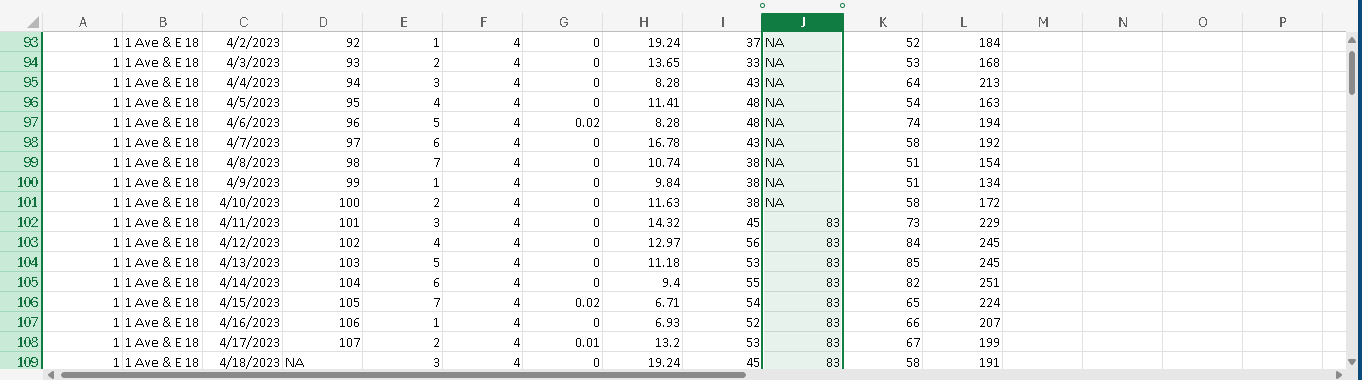
\includegraphics[width=1\linewidth]{excel2.png}
    \caption{Höchste mittlere Temperatur}
    \label{fig:enter-label}
\end{figure}

Die Formel zur Umrechnung von Fahrenheit in Celsius lautet:

\[
T_C = \frac{5}{9} \cdot (T_F - 32)
\]

Setzt man \(T_F = 83\) ein, ergibt sich:

\[
T_C = \frac{5}{9} \cdot (83 - 32) = \frac{5}{9} \cdot 51 = 28{,}33 \,
^\circ\text{c}
\]



Der umgerechnete Wert ist also \(T_C \approx 28.33 \, ^\circ C\).
\newpage
\begin{thebibliography}{9}
\bibitem{Klenke2013} Achim Klenke.
\textit{Wahrscheinlichkeitstheorie}. Springer, 3. Edition, 2013.
\end{thebibliography}

\end{document}
